% answers.tex —— 2011 年·重庆卷·理科 · 参考答案与详细解析片段
% 由 tools/generate_projects.py 依来源总账自 2011/2011_数学真题_重庆理_试题.md + 2011/2011_数学真题_重庆理_解析正文.md + 2011/2011_数学真题_重庆理_答案要点.md 生成，勿手改（改源 MD 后重跑）

\begin{answer}
\gksolhead{1}{}

\textbf{题目}：

复数 $\dfrac{\mathrm i^2+\mathrm i^3+\mathrm i^4}{1-\mathrm i}=$\mbox{（　　）}

（A）$-\frac12-\frac12\mathrm i$

（B）$-\frac12+\frac12\mathrm i$

（C）$\frac12-\frac12\mathrm i$

（D）$\frac12+\frac12\mathrm i$

\Needspace{4\baselineskip}
\textbf{解析}
\nopagebreak[4]
\[\frac{\mathrm i^2+\mathrm i^3+\mathrm i^4}{1-\mathrm i}=\frac{-1-\mathrm i+1}{1-\mathrm i}=\frac{-\mathrm i(1+\mathrm i)}{(1-\mathrm i)(1+\mathrm i)}=\frac{1-\mathrm i}{2}=\frac12-\frac12\mathrm i.\]
选 C。

\gkanswer{答案：C。}

\end{answer}
\begin{answer}
\gksolhead{2}{}

\textbf{题目}：

“$x<-1$”是“$x^2-1>0$”的\mbox{（　　）}

（A）充分而不必要条件

（B）必要而不充分条件

（C）充要条件

（D）既不充分也不必要条件

\Needspace{4\baselineskip}
\textbf{解析}
$x<-1$ 时 $x^2>1$，即 $x^2-1>0$，充分性成立；反之 $x^2-1>0$ 得 $x<-1$ 或 $x>1$，不一定是 $x<-1$。故为充分而不必要条件。选 A。

\gkanswer{答案：A。}

\end{answer}
\begin{answer}
\gksolhead{3}{}

\textbf{题目}：

已知 $\lim\limits_{x\to\infty}\left(\dfrac2{x-1}+\dfrac{ax-1}{3x}\right)=2$，则 $a=$\mbox{（　　）}

（A）$-6$

（B）$2$

（C）$3$

（D）$6$

\Needspace{4\baselineskip}
\textbf{解析}
$x\to\infty$ 时 $\dfrac2{x-1}\to0$，$\dfrac{ax-1}{3x}\to\dfrac a3$，故 $\dfrac a3=2$，$a=6$。选 D。

\gkanswer{答案：D。}

\end{answer}
\begin{answer}
\gksolhead{4}{}

\textbf{题目}：

$(1+3x)^n$（其中 $n\in\mathbf N$ 且 $n\geqslant6$）的展开式中 $x^5$ 与 $x^6$ 的系数相等，则 $n=$\mbox{（　　）}

（A）$6$

（B）$7$

（C）$8$

（D）$9$

\Needspace{4\baselineskip}
\textbf{解析}
\Needspace{5\baselineskip}
$x^5$ 的系数为 $\mathrm C_n^53^5$，$x^6$ 的系数为 $\mathrm C_n^63^6$，由题意
\nopagebreak[4]
\[\mathrm C_n^53^5=\mathrm C_n^63^6\Longrightarrow\frac{\mathrm C_n^6}{\mathrm C_n^5}=3\Longrightarrow\frac{n-5}6=\frac13\Longrightarrow n=7.\]
选 B。

\gkanswer{答案：B。}

\end{answer}
\begin{answer}
\gksolhead{5}{}

\textbf{题目}：

下列区间中，函数 $f(x)=|\ln(2-x)|$ 在其上为增函数的是\mbox{（　　）}

（A）$(-\infty,1]$

（B）$\left[-1,\frac43\right]$

（C）$\left[0,\frac32\right)$

（D）$[1,2)$

\Needspace{4\baselineskip}
\textbf{解析}
定义域为 $x<2$。当 $x<1$ 时 $2-x>1$，$\ln(2-x)>0$，$f(x)=\ln(2-x)$ 递减；当 $1<x<2$ 时 $0<2-x<1$，$\ln(2-x)<0$，$f(x)=-\ln(2-x)$ 递增。故增区间为 $[1,2)$。选 D。

\gkanswer{答案：D。}

\end{answer}
\begin{answer}
\gksolhead{6}{}

\textbf{题目}：

若 $\triangle ABC$ 的内角 $A$，$B$，$C$ 所对的边 $a$，$b$，$c$ 满足 $(a+b)^2-c^2=4$，且 $C=60^\circ$，则 $ab$ 的值为\mbox{（　　）}

（A）$\frac43$

（B）$8-4\sqrt3$

（C）$1$

（D）$\frac23$

\Needspace{4\baselineskip}
\textbf{解析}
\Needspace{5\baselineskip}
由余弦定理 $c^2=a^2+b^2-2ab\cos60^\circ=a^2+b^2-ab$，故
\nopagebreak[4]
\[(a+b)^2-c^2=a^2+2ab+b^2-(a^2+b^2-ab)=3ab=4,\]
即 $ab=\dfrac43$。选 A。

\gkanswer{答案：A。}

\end{answer}
\begin{answer}
\gksolhead{7}{}

\textbf{题目}：

已知 $a>0$，$b>0$，$a+b=2$，则 $y=\dfrac1a+\dfrac4b$ 的最小值是\mbox{（　　）}

（A）$\frac72$

（B）$4$

（C）$\frac92$

（D）$5$

\Needspace{4\baselineskip}
\textbf{解析}
\nopagebreak[4]
\[y=\frac1a+\frac4b=\frac12\left(\frac1a+\frac4b\right)(a+b)=\frac12\left(5+\frac ba+\frac{4a}b\right)\geqslant\frac12\left(5+2\sqrt4\right)=\frac92,\]
当 $\dfrac ba=\dfrac{4a}b$ 即 $b=2a$ 时取等，结合 $a+b=2$ 得 $a=\dfrac23$，$b=\dfrac43$。选 C。

\gkanswer{答案：C。}

\end{answer}
\begin{answer}
\gksolhead{8}{}

\textbf{题目}：

在圆 $x^2+y^2-2x-6y=0$ 内，过点 $E(0,1)$ 的最长弦和最短弦分别为 $AC$ 和 $BD$，则四边形 $ABCD$ 的面积为\mbox{（　　）}

（A）$5\sqrt2$

（B）$10\sqrt2$

（C）$15\sqrt2$

（D）$20\sqrt2$

\Needspace{4\baselineskip}
\textbf{解析}
圆化为 $(x-1)^2+(y-3)^2=10$，圆心 $C_0(1,3)$，半径 $\sqrt{10}$。$|C_0E|=\sqrt{1+4}=\sqrt5<\sqrt{10}$，故 $E$ 在圆内。
\Needspace{5\baselineskip}
最长弦 $AC$ 为过 $E$ 的直径，$|AC|=2\sqrt{10}$；最短弦 $BD$ 为过 $E$ 且垂直于 $C_0E$ 的弦，
\nopagebreak[4]
\[|BD|=2\sqrt{10-5}=2\sqrt5.\]
\Needspace{5\baselineskip}
两弦互相垂直，故
\nopagebreak[4]
\[S_{ABCD}=\frac12|AC|\cdot|BD|=\frac12\cdot2\sqrt{10}\cdot2\sqrt5=10\sqrt2.\]
选 B。

\gkanswer{答案：B。}

\end{answer}
\begin{answer}
\gksolhead{9}{}

\textbf{题目}：

高为 $\dfrac{\sqrt2}4$ 的四棱锥 $S-ABCD$ 的底面是边长为 $1$ 的正方形，点 $S$，$A$，$B$，$C$，$D$ 均在半径为 $1$ 的同一球面上，则底面 $ABCD$ 的中心与顶点 $S$ 之间的距离为\mbox{（　　）}

（A）$\frac{\sqrt2}4$

（B）$\frac{\sqrt2}2$

（C）$1$

（D）$\sqrt2$

\Needspace{4\baselineskip}
\textbf{解析}
\Needspace{5\baselineskip}
设底面中心为原点 $O$，底面在 $z=0$ 内，顶点为 $\left(\pm\dfrac12,\pm\dfrac12,0\right)$，球心在 $z$ 轴上，设为 $(0,0,c)$。由球半径 $1$：
\nopagebreak[4]
\[\frac12+c^2=1\Longrightarrow c=\pm\frac{\sqrt2}2.\]
\Needspace{5\baselineskip}
设 $S(x,y,h)$，$h=\dfrac{\sqrt2}4$。由 $S$ 在球面上：
\nopagebreak[4]
\[x^2+y^2+(h-c)^2=1.\]
\Needspace{5\baselineskip}
若 $c=\dfrac{\sqrt2}2$，则 $h-c=-\dfrac{\sqrt2}4$，$(h-c)^2=\dfrac18$，故 $x^2+y^2=\dfrac78$，于是
\nopagebreak[4]
\[OS^2=x^2+y^2+h^2=\frac78+\frac18=1.\]
若 $c=-\dfrac{\sqrt2}2$，则 $(h-c)^2=\dfrac98>1$，无解。故 $OS=1$。选 C。

\gkanswer{答案：C。}

\end{answer}
\begin{answer}
\gksolhead{10}{}

\textbf{题目}：

设 $m$，$k$ 为整数，方程 $mx^2-kx+2=0$ 在区间 $(0,1)$ 内有两个不同的根，则 $m+k$ 的最小值为\mbox{（　　）}

（A）$-8$

（B）$8$

（C）$12$

（D）$13$

\Needspace{4\baselineskip}
\textbf{解析}
设 $f(x)=mx^2-kx+2$。若 $m<0$，抛物线开口向下且 $f(0)=2>0$，在 $(0,+\infty)$ 上至多一个零点，不合题意，故 $m>0$。
\Needspace{5\baselineskip}
两根都在 $(0,1)$ 内需
\nopagebreak[4]
\[f(0)=2>0,\quad f(1)=m-k+2>0,\quad 0<\frac k{2m}<1,\quad \Delta=k^2-8m>0.\]
即 $k>0$，$k<m+2$，$k^2>8m$。逐一检验：
$m=1$：$k^2>8$ 得 $k\geqslant3$，但 $k<3$，无解；
$m=2$：$k\geqslant5$，但 $k<4$，无解；
$m=3$：$k\geqslant5$，但 $k<5$，无解；
$m=4$：$k\geqslant6$，但 $k<6$，无解；
$m=5$：$k\geqslant7$，但 $k<7$，无解；
$m=6$：$k\geqslant7$ 且 $k<8$，取 $k=7$，此时 $\Delta=1>0$，$\dfrac k{2m}=\dfrac7{12}\in(0,1)$，$f(1)=1>0$，符合。
故 $m+k$ 的最小值为 $6+7=13$。选 D。

\gkanswer{答案：D。}

\end{answer}
\begin{answer}
\gksolhead{11}{}

\textbf{题目}：

在等差数列 $\{a_n\}$ 中，$a_3+a_7=37$，则 $a_2+a_4+a_6+a_8=\underline{\qquad}$。

\Needspace{4\baselineskip}
\textbf{解析}
\Needspace{5\baselineskip}
$a_3+a_7=2a_5=37$，故 $a_5=\dfrac{37}2$。又
\nopagebreak[4]
\[a_2+a_4+a_6+a_8=(a_2+a_8)+(a_4+a_6)=2a_5+2a_5=4a_5=74.\]

\gkanswer{答案：$74$。}

\end{answer}
\begin{answer}
\gksolhead{12}{}

\textbf{题目}：

已知单位向量 $\boldsymbol e_1$，$\boldsymbol e_2$ 的夹角为 $60^\circ$，则 $|2\boldsymbol e_1-\boldsymbol e_2|=\underline{\qquad}$。

\Needspace{4\baselineskip}
\textbf{解析}
\nopagebreak[4]
\[|2\boldsymbol e_1-\boldsymbol e_2|^2=4|\boldsymbol e_1|^2+|\boldsymbol e_2|^2-4\boldsymbol e_1\cdot\boldsymbol e_2=4+1-4\times\frac12=3,\]
故 $|2\boldsymbol e_1-\boldsymbol e_2|=\sqrt3$。

\gkanswer{答案：$\sqrt3$。}

\end{answer}
\begin{answer}
\gksolhead{13}{}

\textbf{题目}：

将一枚均匀的硬币抛掷 $6$ 次，则正面出现的次数比反面出现的次数多的概率为 $\underline{\qquad}$。

\Needspace{4\baselineskip}
\textbf{解析}
\Needspace{5\baselineskip}
正面次数多于反面即正面至少 $4$ 次，
\nopagebreak[4]
\[P=\frac{\mathrm C_6^4+\mathrm C_6^5+\mathrm C_6^6}{2^6}=\frac{15+6+1}{64}=\frac{11}{32}.\]

\gkanswer{答案：$\dfrac{11}{32}$。}

\end{answer}
\begin{answer}
\gksolhead{14}{}

\textbf{题目}：

已知 $\sin\alpha=\dfrac12+\cos\alpha$，且 $\alpha\in\left(0,\dfrac\pi2\right)$，则 $\dfrac{\cos2\alpha}{\sin\left(\alpha-\dfrac\pi4\right)}$ 的值为 $\underline{\qquad}$。

\Needspace{4\baselineskip}
\textbf{解析}
由 $\sin\alpha-\cos\alpha=\dfrac12$ 平方得 $1-\sin2\alpha=\dfrac14$，故 $\sin2\alpha=\dfrac34$。
\Needspace{5\baselineskip}
因 $\alpha\in\left(0,\dfrac\pi2\right)$ 且 $\sin\alpha>\cos\alpha$，故 $\alpha\in\left(\dfrac\pi4,\dfrac\pi2\right)$，$2\alpha\in\left(\dfrac\pi2,\pi\right)$，
\nopagebreak[4]
\[\cos2\alpha=-\sqrt{1-\frac9{16}}=-\frac{\sqrt7}4.\]
\Needspace{5\baselineskip}
又 $\sin\left(\alpha-\dfrac\pi4\right)=\dfrac{\sin\alpha-\cos\alpha}{\sqrt2}=\dfrac{\sqrt2}4$，故
\nopagebreak[4]
\[\frac{\cos2\alpha}{\sin\left(\alpha-\frac\pi4\right)}=\frac{-\frac{\sqrt7}4}{\frac{\sqrt2}4}=-\frac{\sqrt7}{\sqrt2}=-\frac{\sqrt{14}}2.\]

\gkanswer{答案：$-\dfrac{\sqrt{14}}2$。}

\end{answer}
\begin{answer}
\gksolhead{15}{}

\textbf{题目}：

设圆 $C$ 位于抛物线 $y^2=2x$ 与直线 $x=3$ 所围成的封闭区域（包含边界）内，则圆 $C$ 的半径能取到的最大值为 $\underline{\qquad}$。

\Needspace{4\baselineskip}
\textbf{解析}
区域为 $\left\{(x,y)\mid \dfrac{y^2}2\leqslant x\leqslant3\right\}$。由对称性，最大圆圆心为 $(t,0)$，半径 $r=3-t$。
\Needspace{5\baselineskip}
圆心到抛物线 $x=\dfrac{y^2}2$ 的距离：令 $u=y^2\geqslant0$，
\nopagebreak[4]
\[d^2(u)=\left(\frac u2-t\right)^2+u,\]
\Needspace{5\baselineskip}
$d^2$ 在 $u=2t-2$ 处取最小值 $2t-1$（$t\geqslant1$ 时），故圆心到抛物线的距离为 $\sqrt{2t-1}$。由圆在区域内得
\nopagebreak[4]
\[3-t=\sqrt{2t-1}\Longrightarrow(3-t)^2=2t-1\Longrightarrow t^2-8t+10=0,\]
\Needspace{5\baselineskip}
解得 $t=4\pm\sqrt6$。由 $t<3$ 取 $t=4-\sqrt6$，此时
\nopagebreak[4]
\[r=3-t=\sqrt6-1.\]
故最大半径为 $\sqrt6-1$。

\gkanswer{答案：$\sqrt6-1$。}

\end{answer}
\begin{answer}
\gksolhead{16}{}

\textbf{题目}：

设 $a\in\mathbf R$，$f(x)=\cos x(a\sin x-\cos x)+\cos^2\left(\dfrac\pi2-x\right)$ 满足 $f\left(-\dfrac\pi3\right)=f(0)$，求函数 $f(x)$ 在 $\left[\dfrac\pi4,\dfrac{11\pi}{24}\right]$ 上的最大值和最小值。

\Needspace{4\baselineskip}
\textbf{解析}
\Needspace{5\baselineskip}
由 $\cos^2\left(\dfrac\pi2-x\right)=\sin^2x$ 得
\nopagebreak[4]
\[f(x)=a\sin x\cos x-\cos^2x+\sin^2x=\frac a2\sin2x-\cos2x.\]
$f(0)=-1$，$f\left(-\dfrac\pi3\right)=\dfrac a2\cdot\left(-\dfrac{\sqrt3}2\right)-\left(-\dfrac12\right)=-\dfrac{\sqrt3}4a+\dfrac12$。由 $f\left(-\dfrac\pi3\right)=f(0)$ 得 $-\dfrac{\sqrt3}4a+\dfrac12=-1$，故 $a=2\sqrt3$。
\Needspace{5\baselineskip}
于是
\nopagebreak[4]
\[f(x)=\sqrt3\sin2x-\cos2x=2\sin\left(2x-\frac\pi6\right).\]
当 $x\in\left[\dfrac\pi4,\dfrac{11\pi}{24}\right]$ 时，$2x-\dfrac\pi6\in\left[\dfrac\pi3,\dfrac{3\pi}4\right]$。
$\sin$ 在该区间上最大值为 $1$（$2x-\dfrac\pi6=\dfrac\pi2$），最小值在端点取得：$\sin\dfrac\pi3=\dfrac{\sqrt3}2$，$\sin\dfrac{3\pi}4=\dfrac{\sqrt2}2$，最小为 $\dfrac{\sqrt2}2$。
故 $f(x)$ 的最大值为 $2$，最小值为 $\sqrt2$。

\gkanswer{答案：最大值 $2$，最小值 $\sqrt2$。}

\end{answer}
\begin{answer}
\gksolhead{17}{}

\textbf{题目}：

某市公租房的房源位于 $A$，$B$，$C$ 三个片区。设每位申请人只申请其中一个片区的房源，且申请其中任一个片区的房源是等可能的。求该市的任 $4$ 位申请人中：

（1） 恰有 $2$ 人申请 $A$ 片区的房源的概率；

（2） 申请的房源所在片区的个数 $\xi$ 的分布列与期望。

\Needspace{4\baselineskip}
\textbf{解析}
\gksubpart{(1)}
\Needspace{5\baselineskip}
每人申请 $A$ 的概率为 $\dfrac13$，故恰有 $2$ 人申请 $A$ 的概率
\nopagebreak[4]
\[P=\mathrm C_4^2\left(\frac13\right)^2\left(\frac23\right)^2=6\cdot\frac4{81}=\frac8{27}.\]

\gksubpart{(2)}
$\xi$ 的可能取值为 $1,2,3$，总情况数为 $3^4=81$。
$\xi=1$：$4$ 人同去一片区，共 $3$ 种，$P=\dfrac3{81}=\dfrac1{27}$；
\Needspace{5\baselineskip}
$\xi=2$：先选两个片区（$3$ 种），$4$ 人只去这两个片区且都出现，有 $2^4-2=14$ 种，
\nopagebreak[4]
\[P=\frac{3\times14}{81}=\frac{14}{27};\]
\Needspace{5\baselineskip}
$\xi=3$：三个片区都出现，有 $3^4-3\times2^4+3=36$ 种，
\nopagebreak[4]
\[P=\frac{36}{81}=\frac49.\]
\Needspace{5\baselineskip}
故
\nopagebreak[4]
\[E\xi=1\times\frac1{27}+2\times\frac{14}{27}+3\times\frac49=\frac{1+28+36}{27}=\frac{65}{27}.\]

\gkanswer{答案（1）：$\dfrac8{27}$。}

\gkanswer{答案（2）：$\xi$ 的分布列为 $P(\xi=1)=\dfrac1{27}$，$P(\xi=2)=\dfrac{14}{27}$，$P(\xi=3)=\dfrac49$；$E\xi=\dfrac{65}{27}$。}

\end{answer}
\begin{answer}
\gksolhead{18}{}

\textbf{题目}：

设 $f(x)=x^3+ax^2+bx+1$ 的导数 $f'(x)$ 满足 $f'(1)=2a$，$f'(2)=-b$，其中常数 $a$，$b\in\mathbf R$。

（1） 求曲线 $y=f(x)$ 在点 $(1,f(1))$ 处的切线方程；

（2） 设 $g(x)=f'(x)\mathrm e^{-x}$，求函数 $g(x)$ 的极值。

\Needspace{4\baselineskip}
\textbf{解析}
\gksubpart{(1)}
$f'(x)=3x^2+2ax+b$。由 $f'(1)=3+2a+b=2a$ 得 $b=-3$；由 $f'(2)=12+4a+b=-b=3$ 得 $4a=-6$，$a=-\dfrac32$。
\Needspace{5\baselineskip}
$f(1)=1-\dfrac32-3+1=-\dfrac52$，$f'(1)=-3$，故切线为
\nopagebreak[4]
\[y+\frac52=-3(x-1)\Longrightarrow6x+2y-1=0.\]

\gksubpart{(2)}
\Needspace{5\baselineskip}
$f'(x)=3x^2-3x-3$，
\nopagebreak[4]
\[g(x)=3(x^2-x-1)\mathrm e^{-x},\qquad g'(x)=3\left[(2x-1)-(x^2-x-1)\right]\mathrm e^{-x}=-3x(x-3)\mathrm e^{-x}.\]
\Needspace{5\baselineskip}
故 $g$ 在 $(-\infty,0)$ 上递减，在 $(0,3)$ 上递增，在 $(3,+\infty)$ 上递减。于是
\nopagebreak[4]
\[g_{\text{\text{极小}}}=g(0)=-3,\qquad g_{\text{\text{极大}}}=g(3)=15\mathrm e^{-3}.\]

\gkanswer{答案（1）：$6x+2y-1=0$。}

\gkanswer{答案（2）：极小值 $-3$（$x=0$），极大值 $15\mathrm e^{-3}$（$x=3$）。}

\end{answer}
\begin{answer}
\gksolhead{19}{}

\textbf{题目}：

如图，在四面体 $ABCD$ 中，平面 $ABC\perp$ 平面 $ACD$，$AB\perp BC$，$AD=CD$，$\angle CAD=30^\circ$。

（1） 若 $AD=2$，$AB=2BC$，求四面体 $ABCD$ 的体积；

（2） 若二面角 $C-AB-D$ 为 $60^\circ$，求异面直线 $AD$ 与 $BC$ 所成角的余弦值。
\nopagebreak[4]
\begin{center}% 2011 年重庆卷理科第 19 题：四面体 ABCD，平面 ABC⊥平面 ACD。
% 来源 PDF：普通高考/2011/2011重庆理.pdf，SHA-256 15c5e4dfbc23f3b3e1c37b279db7aea1a8e3db05ea86087e2346208274bc7ef7。
% 原页：第 2 页第 1 栏上部，书页码 652。示意。
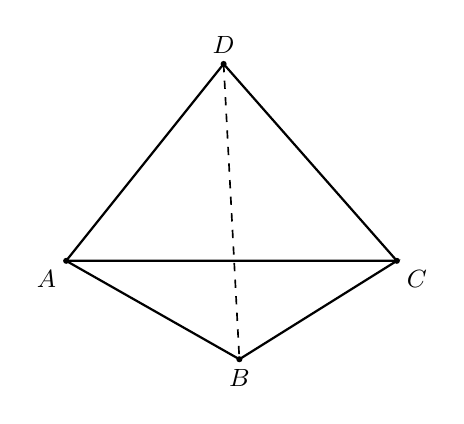
\begin{tikzpicture}[>=stealth, semithick, font=\small, scale=1.0]
  \coordinate (A) at (0,0);
  \coordinate (C) at (4.2,0);
  \coordinate (B) at (2.2,-1.25);
  \coordinate (D) at (2.0,2.5);
  \draw[thick] (A)--(B)--(C)--(A);
  \draw[thick] (D)--(A) (D)--(C);
  \draw[dashed] (D)--(B);
  \fill (A) circle (1.1pt) node[below left] {$A$};
  \fill (B) circle (1.1pt) node[below] {$B$};
  \fill (C) circle (1.1pt) node[below right] {$C$};
  \fill (D) circle (1.1pt) node[above] {$D$};
\end{tikzpicture}
\end{center}
\nopagebreak[4]
\Needspace{4\baselineskip}
\textbf{解析}
设 $AC$ 在 $x$ 轴上，$A(0,0,0)$，平面 $ACD$ 为 $z=0$，由平面 $ABC\perp$ 平面 $ACD$ 可设 $B(x,0,z)$。
\Needspace{5\baselineskip}
由 $AD=CD$ 且 $\angle CAD=30^\circ$，点 $D$ 在 $AC$ 的垂直平分线上；设 $D$ 到 $AC$ 的距离为 $t>0$，则
\nopagebreak[4]
\[D(\sqrt3t,t,0),\qquad C(2\sqrt3t,0,0),\]
\gksubpart{(1)}
$AD=2$ 即 $2t=2$，$t=1$，$AC=2\sqrt3$，$D(\sqrt3,1,0)$，$S_{\triangle ACD}=\dfrac12\cdot2\sqrt3\cdot1=\sqrt3$。
$AB\perp BC$ 且 $AB=2BC$，由 $AC^2=AB^2+BC^2=5BC^2=12$ 得 $BC=\dfrac{2\sqrt3}{\sqrt5}$，$AB=\dfrac{4\sqrt3}{\sqrt5}$。
\Needspace{5\baselineskip}
$B$ 到 $AC$ 的距离为 $\dfrac{AB\cdot BC}{AC}=\dfrac{4\sqrt3/5}{2\sqrt3}=\dfrac45$，即 $B$ 到平面 $ACD$ 的距离为 $\dfrac45$。故
\nopagebreak[4]
\[V=\frac13\cdot\sqrt3\cdot\frac45=\frac45.\]

\gksubpart{(2)}
由 $AB\perp BC$ 得 $(x-2\sqrt3t)x+z^2=0$，即 $x^2+z^2=2\sqrt3tx$。
\Needspace{5\baselineskip}
平面 $ABC$ 的法向量为 $(0,1,0)$；平面 $ABD$ 的法向量
\nopagebreak[4]
\[\boldsymbol n=\overrightarrow{AB}\times\overrightarrow{AD}=(x,0,z)\times(\sqrt3t,t,0)=(-zt,\sqrt3tz,xt).\]
\Needspace{5\baselineskip}
二面角 $C-AB-D$ 为 $60^\circ$，故
\nopagebreak[4]
\[\frac{\sqrt3tz}{t\sqrt{z^2+3z^2+x^2}}=\frac{\sqrt3z}{\sqrt{4z^2+x^2}}=\frac12\Longrightarrow x^2=8z^2.\]
\Needspace{5\baselineskip}
代入 $x^2+z^2=2\sqrt3tx$ 得 $9z^2=2\sqrt3tx$，结合 $x=2\sqrt2z$ 解得
\nopagebreak[4]
\[z=\frac{4\sqrt6}9t,\qquad x=\frac{16\sqrt3}9t.\]
\Needspace{5\baselineskip}
于是
\nopagebreak[4]
\[\overrightarrow{AD}=(\sqrt3t,t,0),\qquad \overrightarrow{BC}=\left(\frac{2\sqrt3}9t,0,-\frac{4\sqrt6}9t\right),\]
\nopagebreak[4]
\[|\overrightarrow{AD}|=2t,\qquad |\overrightarrow{BC}|=\frac{2\sqrt3}3t,\qquad \overrightarrow{AD}\cdot\overrightarrow{BC}=\frac23t^2,\]
\Needspace{5\baselineskip}
故异面直线 $AD$ 与 $BC$ 所成角的余弦值为
\nopagebreak[4]
\[\cos\theta=\frac{\frac23t^2}{2t\cdot\frac{2\sqrt3}3t}=\frac{\sqrt3}6.\]

\gkanswer{答案（1）：$\dfrac45$。}

\gkanswer{答案（2）：$\dfrac{\sqrt3}6$。}

\end{answer}
\begin{answer}
\gksolhead{20}{}

\textbf{题目}：

如图，椭圆的中心为原点 $O$，离心率 $e=\dfrac{\sqrt2}2$，一条准线的方程为 $x=2\sqrt2$。

（1） 求该椭圆的标准方程；

（2） 设动点 $P$ 满足 $\overrightarrow{OP}=\overrightarrow{OM}+2\overrightarrow{ON}$，其中 $M$，$N$ 是椭圆上的点，直线 $OM$ 与 $ON$ 的斜率之积为 $-\dfrac12$。问：是否存在两个定点 $F_1$，$F_2$，使得 $|PF_1|+|PF_2|$ 为定值？若存在，求 $F_1$，$F_2$ 的坐标；若不存在，说明理由。
\nopagebreak[4]
\begin{center}% 2011 年重庆卷理科第 20 题：椭圆、准线 x=2√2 与点 P、M、N。
% 来源 PDF：普通高考/2011/2011重庆理.pdf，SHA-256 15c5e4dfbc23f3b3e1c37b279db7aea1a8e3db05ea86087e2346208274bc7ef7。
% 原页：第 2 页第 2 栏中部，书页码 652。示意。
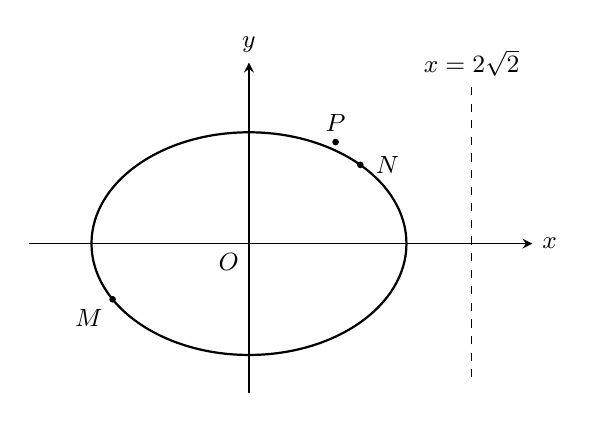
\begin{tikzpicture}[>=stealth, semithick, font=\small, scale=1.0]
  \draw[->] (-2.8,0)--(3.6,0) node[right] {$x$};
  \draw[->] (0,-1.9)--(0,2.3) node[above] {$y$};
  \draw[thick] (0,0) ellipse (2 and 1.414);
  \draw[dashed] (2.828,-1.7)--(2.828,2.0) node[above] {$x=2\sqrt2$};
  \fill (-1.732,-0.707) circle (1.2pt) node[below left] {$M$};
  \fill (1.414,1.0) circle (1.2pt) node[right=2pt] {$N$};
  \fill (1.10,1.29) circle (1.2pt) node[above] {$P$};
  \node[below left] at (0,0) {$O$};
\end{tikzpicture}
\end{center}
\nopagebreak[4]
\Needspace{4\baselineskip}
\textbf{解析}
\gksubpart{(1)}
设椭圆为 $\dfrac{x^2}{a^2}+\dfrac{y^2}{b^2}=1$，$e=\dfrac ca=\dfrac{\sqrt2}2$，准线 $x=\dfrac{a^2}c=2\sqrt2$。
\Needspace{5\baselineskip}
由 $c=\dfrac a{\sqrt2}$ 得 $a^2/c=a\sqrt2=2\sqrt2$，故 $a=2$，$c=\sqrt2$，$b^2=a^2-c^2=2$。椭圆为
\nopagebreak[4]
\[\frac{x^2}4+\frac{y^2}2=1.\]

\gksubpart{(2)}
\Needspace{5\baselineskip}
设 $M(2\cos\alpha,\sqrt2\sin\alpha)$，$N(2\cos\beta,\sqrt2\sin\beta)$，则
\nopagebreak[4]
\[k_{OM}k_{ON}=\frac{\sqrt2\sin\alpha}{2\cos\alpha}\cdot\frac{\sqrt2\sin\beta}{2\cos\beta}=\frac12\tan\alpha\tan\beta=-\frac12,\]
故 $\tan\alpha\tan\beta=-1$，即 $\beta=\alpha\pm\dfrac\pi2$。
\Needspace{5\baselineskip}
不妨取 $\beta=\alpha+\dfrac\pi2$，则 $\cos\beta=-\sin\alpha$，$\sin\beta=\cos\alpha$，于是
\nopagebreak[4]
\[P=M+2N=(2\cos\alpha-4\sin\alpha,\ \sqrt2\sin\alpha+2\sqrt2\cos\alpha).\]
\Needspace{5\baselineskip}
记 $s=\sin\alpha$，$c_0=\cos\alpha$，则
\nopagebreak[4]
\[\frac{x_P^2}{20}+\frac{y_P^2}{10}=\frac{(2c_0-4s)^2}{20}+\frac{2(s+2c_0)^2}{10}
=\frac{4c_0^2-16c_0s+16s^2+4s^2+16c_0s+16c_0^2}{20}=1.\]
\Needspace{5\baselineskip}
故 $P$ 在椭圆 $\dfrac{x^2}{20}+\dfrac{y^2}{10}=1$ 上，其焦点为 $F_1(-\sqrt{10},0)$，$F_2(\sqrt{10},0)$，且
\nopagebreak[4]
\[|PF_1|+|PF_2|=2\sqrt{20}=4\sqrt5\]
为定值。$\beta=\alpha-\dfrac\pi2$ 时同理。故存在满足条件的定点 $F_1(-\sqrt{10},0)$，$F_2(\sqrt{10},0)$。

\gkanswer{答案（1）：$\dfrac{x^2}4+\dfrac{y^2}2=1$。}

\gkanswer{答案（2）：存在，$F_1(-\sqrt{10},0)$，$F_2(\sqrt{10},0)$，$|PF_1|+|PF_2|=4\sqrt5$。}

\end{answer}
\begin{answer}
\gksolhead{21}{}

\textbf{题目}：

设实数数列 $\{a_n\}$ 的前 $n$ 项和 $S_n$ 满足 $S_{n+1}=a_{n+1}S_n$（$n\in\mathbf N^*$）。

（1） 若 $a_1$，$S_2$，$-2a_2$ 成等比数列，求 $S_2$ 和 $a_3$；

（2） 求证：对 $k\geqslant3$ 有 $0\leqslant a_{k+1}\leqslant a_k\leqslant\dfrac43$。

\Needspace{4\baselineskip}
\textbf{解析}
\gksubpart{(1)}
由 $S_{n+1}=a_{n+1}S_n$ 取 $n=1$ 得 $S_2=a_2S_1=a_1a_2$；又 $S_2=a_1+a_2$，故 $a_1a_2=a_1+a_2$。
$a_1$，$S_2$，$-2a_2$ 成等比数列，故 $S_2^2=-2a_1a_2$。记 $p=a_1a_2=S_2$，则 $p^2=-2p$，$p=0$ 或 $p=-2$。
若 $p=0$，则 $a_1+a_2=0$ 且 $a_1a_2=0$，得 $a_1=a_2=0$，此时 $a_1=0$ 不能作等比数列的首项，舍去。
故 $S_2=p=-2$，且 $a_1+a_2=-2$，$a_1a_2=-2$。
由 $S_3=a_3S_2$ 得 $a_1+a_2+a_3=-2a_3$，即 $-2+a_3=-2a_3$，故 $a_3=\dfrac23$。

\gksubpart{(2)}
\Needspace{5\baselineskip}
由 (1) $S_2=-2<0$。设 $S_n<0$，由 $S_{n+1}=a_{n+1}S_n$ 及 $S_{n+1}=S_n+a_{n+1}$ 得
\nopagebreak[4]
\[a_{n+1}=\frac{S_n}{S_n-1},\qquad S_{n+1}=\frac{S_n^2}{S_n-1}<0,\]
故对一切 $n\geqslant2$ 有 $S_n<0$。
\Needspace{5\baselineskip}
令 $t_n=-S_n>0$（$n\geqslant2$），则
\nopagebreak[4]
\[t_{n+1}=\frac{t_n^2}{t_n+1}<t_n,\qquad a_{n+1}=\frac{t_n}{t_n+1}.\]
\Needspace{5\baselineskip}
于是 $a_{n+1}\in(0,1)\subset\left[0,\dfrac43\right]$，且 $t\mapsto\dfrac t{t+1}$ 在 $(0,+\infty)$ 上递增，由 $t_{n+1}<t_n$ 得
\nopagebreak[4]
\[a_{n+2}=\frac{t_{n+1}}{t_{n+1}+1}<\frac{t_n}{t_n+1}=a_{n+1}.\]
取 $n=k-1$（$k\geqslant3$）即得 $0\leqslant a_{k+1}<a_k<1\leqslant\dfrac43$，故所证不等式成立。

\gkanswer{答案（1）：$S_2=-2$，$a_3=\dfrac23$。}

\gkanswer{答案（2）：证明见解析。}

\end{answer}